\documentclass{article}
\usepackage{amssymb, amsmath, booktabs, caption}
\usepackage[margin=1in]{geometry}
\usepackage{tikz, pgfplots}
\usetikzlibrary{shapes,arrows}
\pgfmathdeclarefunction{gauss}{2}{%
  \pgfmathparse{1/(#2*sqrt(2*pi))*exp(-((x-#1)^2)/(2*#2^2))}%
}

\title{Econometrics Final Concepts}
\author{Ryan Safner}
\date{Fall 2017}

\begin{document}
	
\maketitle

\section*{Ordinary Least Squares (OLS) Regression}

\begin{itemize}
	\item	Bivariate data and associations between variables (e.g. $X$ and $Y$)
	\begin{itemize}
		\item Apparent relationships are best viewed by looking at a scatterplot
		\begin{itemize}
			\item Check for associations to be positive/negative, weak/strong, linear/nonlinear, etc
			\item $Y$: dependent variable
			\item $X$: independent variable 
		\end{itemize}
		\item Correlation coefficient ($r$) can quantify the strength of an association
		\begin{equation*}
					r=\frac{1}{n-1} \sum^n \bigg(\frac{X_i-\bar{X}}{s_X}\bigg) \bigg(\frac{Y_i-\bar{Y}}{s_Y}\bigg) = \frac{\displaystyle \sum^n Z_X Z_Y}{n-1}	
		\end{equation*}
		\begin{itemize}
			\item $-1 \leq r \leq 1$ and $r$ only measures \emph{linear} associations
			\item $|r|$ closer to 1 imply stronger correlation (near a perfect straight line)  
			\item Correlation does not imply causation! Might be confounding or lurking variables (e.g. $Z$) affecting $X$ and/or $Y$
		\end{itemize}
	\end{itemize}
	\item Population regression model
	\begin{equation*}
Y_i=\beta_0+\beta_1X_i+\epsilon_i
	\end{equation*}
	\begin{itemize}
		\item $\beta_1$: $\frac{\Delta Y}{\Delta X}$: the slope between $X$ and $Y$, number of units of $Y$ from a 1 unit change in $X$ 
		\item $\beta_0$ is the $Y$-intercept: literally, value of $Y$ when $X=0$
		\item $\epsilon_i$ is the error or residual, difference between actual value of $Y|X$ vs. predicted value of $\hat{Y}$
	\end{itemize}
		\begin{figure}[h!]
			\centering 
				\begin{tikzpicture}[scale=.75]\small  
				\draw[->] (0,0) -- (11,0) coordinate (x axis) node[right]{$X$};
 				\draw[->] (0,0) -- (0,11) coordinate (y axis) node[above]{$Y$};	
            	\draw[ultra thick, dashed, red] (5,5)--node[right]{$\epsilon_i = Y_i-\hat{Y}_i$}(5,6.75);
            	\draw[fill=black](1,4) circle(0.125cm);
            	\draw[fill=black](2,6) circle(0.125cm);
            	\draw[fill=black](4,2) circle(0.125cm);
            	\draw[fill=black](4,7) circle(0.125cm);
            	\draw[fill=black](5,5) circle(0.125cm)node[below]{($X_i,Y_i)$};
            	\draw[fill=black](5,5) circle(0.125cm);
            	\draw[fill=black](6,8) circle(0.125cm);
            	\draw[fill=black](7,9) circle(0.125cm);
            	\draw[fill=black](8,9) circle(0.125cm);
            	\draw[fill=black](9,10) circle(0.125cm);
            	\draw[fill=black](3,8) circle(0.125cm);
            	\draw[ultra thick, blue] (0,3)node[left]{$\beta_0$}--(9.5,10)node[right]{$\hat{Y}=\beta_0+\beta_1 X$};
            	\draw[very thick, blue, dashed] (7,8)--node[below]{$1$}(8,8)--node[right]{$\beta_1$}(8,9);
            	\draw[thick, dotted] (0,5)node[left]{$Y_i$}--(5,5)--(5,0)node[below]{$X_i$};
            	\draw[thick, dotted] (0,6.75)node[left]{$\hat{Y_i}$}--(5,6.75);
 			\end{tikzpicture}	
	\end{figure}
	\item Ordinary Least Squares (OLS) regression model 
		\begin{equation*}
\hat{Y_i}=\hat{\beta_0}+\hat{\beta_1}X_i
		\end{equation*}
	\begin{itemize}
		\item Least square estimators $\hat{\beta_0}$ and $\hat{\beta_1}$ estimate population regression line from sample data
		\item Minimize sum of squared errors (SSE) $min\displaystyle \sum^n \epsilon_i^2$ where $\epsilon_i=Y_i-\hat{Y_i}$
		\item OLS regression line
		\begin{equation*}
 \hat{\beta_1} = \frac{cov(X,Y)}{var(X)}=\frac{\sum (X_i-\bar{X})(Y_i-\bar{Y})}{\sum (X_i-\bar{X})^2}=r_{X,Y}\frac{s_Y}{s_X}
		\end{equation*}
		\begin{equation*}
\hat{\beta_0} = \bar{Y}-\hat{\beta_1}\bar{X}		\end{equation*}
		\end{itemize}
\clearpage 
	\item Measures of Fit
	\begin{itemize}
		\item $R^2$: fraction of total variation on $Y$ explained by variation in $X$ according to model
		\begin{equation*}
		R^2=\frac{ESS}{TSS}	
		\end{equation*}
		\begin{equation*}
		R^2=1-\frac{SSE}{TSS}	
		\end{equation*}
		\begin{equation*}
		R^2=r_{X,Y}^2	
		\end{equation*}
		\begin{itemize}
			\item $ESS = \sum (\hat{Y_i}-\bar{Y})^2$
			\item $TSS = \sum(Y_i-\bar{Y})^2$
			\item $SSE = \sum \hat{\epsilon_i}^2$ 
		\end{itemize}
		\item Standard error of the regression (SER): average size of $\epsilon_i$, average distance from regression line to data points
		\begin{equation*}
		SER=\frac{1}{n-2}\sum \hat{\epsilon_i}^2 = \frac{SSE}{n-2}
		\end{equation*}
	\end{itemize}
	\item Hypothesis testing of $\beta_1$
	\begin{itemize}
		\item $H_0: \beta_1=\beta_{1,0}$, often $H_0: \beta_1=0$
		\item Two sided alternative $H_1: \beta_1 \neq 0$
		\item One sided alternatives $H_1: \beta_1 > 0$, $H_2: \beta_1 < 0$
		\item $t$-statistic
		\begin{equation*}
t=\frac{\hat{\beta_1}-\beta_{1,0}}{SE[\hat{\beta_1}]}
		\end{equation*}
		\item Compare $t$ against critical value $t$*, or compute $p$-value as usual 
		\item Confidence intervals (95\%): $\hat{\beta_1} \pm 1.96(SE[\hat{\beta_1}])$
	\end{itemize}
			\begin{figure}[h!]
		\centering 	
			\begin{tikzpicture}\scriptsize 
\begin{axis}[
  no markers, domain=-4:4, samples=100,
  axis lines*=left, xlabel=$\hat{\beta_1}$, ylabel={},
  every axis y label/.style={at=(current axis.above origin),anchor=south},
  every axis x label/.style={at=(current axis.right of origin),anchor=west},
  height=5cm, width=10cm,
  xtick=\empty, ytick=\empty,
  enlargelimits=false, clip=false, axis on top,
  %grid = major
  ]
  \addplot [very thick,cyan!50!black] {gauss(0,0.5)};
  \draw [yshift=0cm, thick, dashed](axis cs:0,0)node[below]{$\beta_1$}--(axis cs:0,0.8);
  \draw[cyan!50!black](axis cs:1,0.8)node[above]{Small variance};
    \addplot [very thick,red!50!black] {gauss(0,1.5)};
  \draw[red!50!black](axis cs:2,0.3)node[above]{Large variance};
\end{axis}
\end{tikzpicture}
\caption*{\small $\hat{\beta_1}$ is a random variable, so it has its own sampling distribution with mean $E[\hat{\beta_1}]$ and standard error $se[\hat{\beta_1}]$}
	\end{figure}
	\item Mean of OLS estimator $\hat{\beta_1}$ \& Bias: Endogeneity \& Exogeneity
	\begin{itemize}
		\item $X$ is \textbf{exogenous} if it is not correlated with the error term 
	\begin{equation*}
 	corr(X, \epsilon)=0
 	\end{equation*}
		\begin{itemize}
			\item Equivalently, knowing $X$ should not give you any information about $\epsilon$:
				\begin{equation*}
 	E[\epsilon|X]=0
 	\end{equation*}
			\item If $X$ is exogenous, OLS estimate on $X$ is unbiased: 
							\begin{equation*}
 	E[\hat{\beta_1}]=\beta_1
 	\end{equation*}
		\end{itemize}
		\item $X$ is \textbf{endogenous} if it is correlated with the error term
	\begin{equation*}
 	corr(X, \epsilon) \neq 0
 	\end{equation*}
		\begin{itemize}
			\item Equivalently, knowing $X$ gives you information about $\epsilon$: 
				\begin{equation*}
 	E[\epsilon|X] \neq 0
 	\end{equation*}
			\item If $X$ is endogenous, OLS estimate on $X$ is biased: 
			\begin{equation*}
E[\hat{\beta_1}]=\beta_1+corr(X,\epsilon)\frac{\sigma_\epsilon}{\sigma_X}
		\end{equation*}
			\begin{itemize}
				\item Can measure strength and direction ($+$ or $-$) of bias 
				\item Note: if unbiased, $corr(X,\epsilon)=0$, so $E[\hat{\beta_1}]=\beta_1$
			\end{itemize}
		\end{itemize}
	\end{itemize}  
	\item Variance of OLS estimator $\hat{\beta_1}$, measuring precision of estimate
			\begin{equation*}
		var[\hat{\beta_1}]=\frac{\hat{\sigma}^2}{n\times var(X)}
		\end{equation*}
		and standard error 
	\begin{equation*}
		se[\hat{\beta_1}]=\sqrt{\frac{\hat{\sigma}^2}{n\times var(X)}}
		\end{equation*}
	\begin{itemize}
	\item Affected by 3 major factors: 
	\begin{enumerate}
		\item Model fit, where SER=$\hat{\sigma}$
		\item Sample size $n$
		\item Variation in $X_j$
	\end{enumerate}
	\end{itemize}
	\item Heteroskedasticity and homoskedasticity
	\begin{itemize}
		\item Homoskedastic errors ($\epsilon$) have the same variance over all values of $X$
		\item Heteroskedastic errors ($\epsilon$) have different variance over values of $X$
		\begin{itemize}
			\item Heteroskedasticity does \emph{not} bias our estimates, but incorrectly lowers variance \& standard errors (inflating $t$-statistics and significance!) 
			\item Can correct for heteroskedasticity by using robust standard errors 
		\end{itemize}
	\end{itemize} 
\end{itemize}

\clearpage 

\section*{Multivariate Regression}

\begin{itemize}
	\item Omitted Variable Bias 
	\begin{itemize}
		\item A variable $Z$ causes omitted variable bias if: 
		\begin{enumerate}
			\item $corr(X,Z) \neq 0$, $X$ and $Z$ are correlated
			\item $corr(Z, Y) \neq 0$, $Z$ is in the error term that explains $Y$	
		\end{enumerate}
		\item Omitted variable bias can be avoided by including $Z$ in the regression (as $X_2$) 
	\end{itemize}	
	\item Multivariate Regression Model
	\begin{equation*}
	\widehat{Y_i}=\hat{\beta_0}+\hat{\beta_1}X_{1i}+\hat{\beta_2}X_{2i}+\hat{\epsilon_i}	
	\end{equation*}
	\begin{itemize}
		\item $\hat{\beta_0}$: predicted value of $\hat{Y_i}$ when $X_{1i}=0; X_{2i}=0$
		\item $\hat{\beta_1}=\displaystyle\frac{\Delta Y_i}{\Delta X_{1i}}$, marginal effect of $X_{1i}$ on $Y_i$, holding $X_{2i}$ constant
		\item $\hat{\beta_2}=\displaystyle\frac{\Delta Y_i}{\Delta X_{2i}}$, marginal effect of $X_{2i}$ on $Y_i$, holding $X_{1i}$ constant
	\end{itemize} 
	\item Measuring Omitted Variable Bias
	\begin{itemize}
		\item Suppose we omit $X_{2i}$ and run an Omitted Regression
		\begin{equation*}
	Y_i=\alpha_0+\alpha_1X_{1i}+\nu_{i}	
		\end{equation*}
		\item If we run an Auxiliary Regression of $X_{2i}$ on $X_{1i}$:
		\begin{equation*}
			X_{2i}=\delta_0+\delta_1 X_{1i}+\tau_i	
		\end{equation*}
		\begin{itemize}
			\item Size and significance of $\delta_1$ measures relationship between $X_{1i}$ and $X_{2i}$
		\end{itemize}
		\begin{equation*}
		\alpha_1 = \beta_1 + \beta_2 \delta_1
		\end{equation*}
		\item Biased estimate $\alpha_1$ in Omitted Regression picks up:
		\begin{itemize}
			\item True effect of $X_{1i}$ on $Y_i$ ($\beta_1$)
			\item Effect of $X_{2i}$ on $Y_i$ ($\beta_2)$ as pulled through the relationship between $X_{1i}$ and $X_{2i}$ ($\delta_1$)
		\end{itemize}
		\item Conditions for $Z$ being an omitted variable 
		\begin{itemize}
			\item $Z_i$ must be a determinant of $Y_i$ ($\beta_2 \neq 0$)
			\item $Z_i$ is correlated with $X_{1i}$ ($\delta_1 \neq 0$)
		\end{itemize}
	\end{itemize}
			\begin{figure}[h!]
		\centering 	
			\begin{tikzpicture}\scriptsize 
\begin{axis}[
  no markers, domain=-4:4, samples=100,
  axis lines*=left, xlabel=$\hat{\beta_j}$, ylabel={},
  every axis y label/.style={at=(current axis.above origin),anchor=south},
  every axis x label/.style={at=(current axis.right of origin),anchor=west},
  height=5cm, width=10cm,
  xtick=\empty, ytick=\empty,
  enlargelimits=false, clip=false, axis on top,
  %grid = major
  ]
  \addplot [very thick,cyan!50!black] {gauss(0,0.5)};
  \draw [yshift=0cm, thick, dashed](axis cs:0,0)node[below]{$\beta_j$}--(axis cs:0,0.8);
  \draw[cyan!50!black](axis cs:1,0.8)node[above]{Small variance};
    \addplot [very thick,red!50!black] {gauss(0,1.5)};
  \draw[red!50!black](axis cs:2,0.3)node[above]{Large variance};
\end{axis}
\end{tikzpicture}
\caption*{\small $\hat{\beta_j}$ is a random variable, so it has its own sampling distribution with mean $E[\hat{\beta_j}]$ and standard error $se[\hat{\beta_j}]$}
	\end{figure}
	\item Variance of OLS estimators $\hat{\beta_j}$
			\begin{equation*}
		var[\hat{\beta_j}]=\frac{1}{(1-R^2_j)}*\frac{\hat{\sigma}^2}{n\times var[X_j]}
		\end{equation*}
	and Standard error 
		\begin{equation*}
		s.e.[\hat{\beta_j}]=\sqrt{var[\hat{\beta_j}]}
		\end{equation*}
	\item Affected by 4 major factors: 
	\begin{enumerate}
		\item Model fit, where SER=$\hat{\sigma}$
		\item Sample size $n$
		\item Variation in $X_j$
		\item Variance Inflation Factor (VIF) $\frac{1}{1-R^2_j}$
		\begin{itemize}
			\item Independent variables are \textbf{multicollinear} if they are correlated 
			\begin{equation*}
				corr(X_j, X_l) \neq 0 \text{ for } j \neq l
			\end{equation*}
			\item Does not bias estimators, but increases their variance \& standard errors 
			\item $R^2_j$ is the $R^2$ from an auxiliary regression of $X_j$ on all other regressors
			\item VIF quantifies how by many times the variance of $\hat{\beta_j}$ increased because of multicollinearity
			\begin{itemize}
				\item $VIF>10$ (or $\frac{1}{VIF}>0.10$) is bad 
			\end{itemize}
			\item \textbf{Perfect multicollinearity} when a regressor is an exact linear function of (an)other regressor(s) -- cannot run a regression, a logical impossibility 
			\begin{equation*}
			|corr(X_1, X_2)| = 1	
			\end{equation*}
		\end{itemize}
	\end{enumerate}
\end{itemize}

\clearpage 

\section*{Dummy Variables}

\begin{itemize}
	\item Dummy variable 		\[D_i = \left\{
 		 \begin{array}{ll}
    		1 & \text{if } i \text{ meets  condition} \\
   			0 & \text{if } i \text{ does not meet condition }\\
  		\end{array}
  		\right.
		\]
	\item Dummy variables measure group means 
		\begin{equation*}
	\hat{Y_i}=\hat{\beta_0}+\hat{\beta_1} D_i
	\end{equation*}
	\begin{itemize}
		\item When $D_i=0$ (Control group):
		\begin{itemize}
			\item $\hat{Y_i}=\hat{\beta_0}$
			\item $E[Y|D_i=0]=\hat{\beta_0}$ $\iff$ the mean of $Y$ when $D_i=0$
		\end{itemize}
		\item When $D_i=1$ (Treatment group):
		\begin{itemize}
			\item $\hat{Y_i}=\hat{\beta_0}+\hat{\beta_1} D_i$
			\item $E[Y|D_i=1]=\hat{\beta_0}+\hat{\beta_1}$ $\iff$ the mean of $Y$ when $D_i=1$
		\end{itemize}
		\item Difference in group means:
		\begin{align*}
		&=E[Y_i|D_i=1]-E[Y_i|D_i=0]\\
		&=(\hat{\beta_0}+\hat{\beta_1})-(\hat{\beta_0})\\
		&=\hat{\beta_1}\\
		\end{align*}
	\end{itemize}
	\item Transforming categorical variables into dummies 
	\begin{itemize}
		\item A categorical variable (e.g. region, class standing, etc) can be added to a regression by making each category option a dummy variable and including them all (minus one) 
		\begin{equation*}
		Y_i=\beta_0+\beta_2 D_1 + \beta_2 D_2 + \beta_3 D_3	
		\end{equation*}
		where observations can fall into category 1, 2, 3, or 4
		\item Including all category option dummies into a regression yields the \textbf{dummy variable trap}, where all dummies are perfectly multicollinear
		\item Must drop one category dummy, the ``reference group''
		\item Coefficients on dummy variables are the difference between that category and the reference category: 
		\begin{itemize}
			\item $\beta_0=Y$ for category 4 (omitted)
			\item $\beta_1=$ difference between category 1 and category 4 (omitted)
			\item $\beta_2=$ difference between category 2 and category 4 (omitted)
			\item $\beta_3=$ difference between category 3 and category 4 (omitted)
	\end{itemize}
	\end{itemize}
	\item \textbf{Interaction terms} measure if there is an additional effect of one variable on the value of another, 3 combinations:
	\begin{enumerate}
		\item Between a dummy and a continuous variable 
		\begin{equation*}
		Y_i=\beta_0+\beta_1X_i+\beta_2 D_i+\beta_3 \mathbf{X_i \times D_i}
		\end{equation*}
		\begin{itemize}
		\item Coefficients: 
		\begin{itemize}
			\item $\beta_0$: $Y_i$ for $X_i=0$ and $D_i=0$
			\item $\beta_1$: Effect of $X_i \rightarrow Y_i$ for $D_i=0$
			\item $\beta_2$: Effect on $Y_i$ of difference between $D_i=0$ and $D_i=1$
			\item $\beta_3$: Effect of \emph{difference} of $X_i \rightarrow Y_i$ between $D_i=0$ and $D_i=1$
		\end{itemize} 
		\item Easier to see as two different regression lines: 
		\begin{itemize}
		\item When $D_i=0$ (Control group):
			\begin{equation*}
			\textcolor{magenta}{\hat{Y_i} =\hat{\beta_0}+\hat{\beta_1}X_i}
			\end{equation*}
		\item When $D_i=1$ (Treatment group):
			\begin{equation*}
			\textcolor{teal}{\hat{Y_i} =(\hat{\beta_0}+\hat{\beta_2})+(\hat{\beta_1}+\hat{\beta_3})X_i}
			\end{equation*}
			\begin{figure}[h!]
				\centering 
				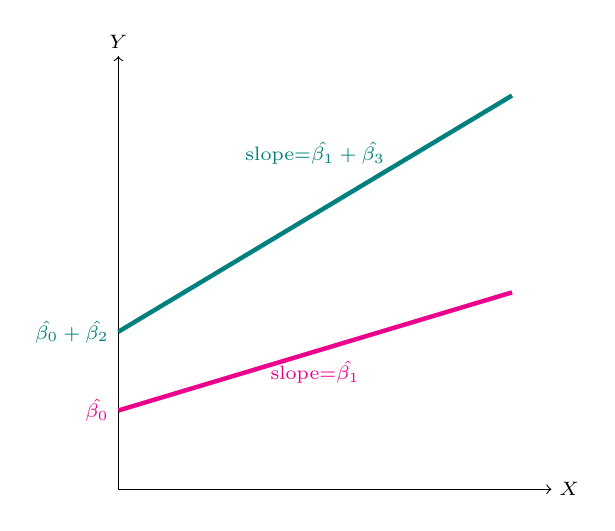
\begin{tikzpicture}[scale=.5]\scriptsize 
				\draw[->] (0,0) -- (11,0) coordinate (x axis) node[right]{$X$};
 				\draw[->] (0,0) -- (0,11) coordinate (y axis) node[above]{$Y$};	
            	\draw[ultra thick, magenta] (0,2)node[left]{$\hat{\beta_0}$}--node[below]{slope=$\hat{\beta_1}$}(10,5);
            	\draw[ultra thick, teal] (0,4)node[left]{$\hat{\beta_0}+\hat{\beta_2}$}--node[above=.5cm]{slope=$\hat{\beta_1}+\hat{\beta_3}$}(10,10);
 			\end{tikzpicture}	
	\end{figure}
 			\item Two regression lines may have (same/different) intercepts and (same/different) intercepts, test significance of: 
 			\begin{itemize}
 				\item $\beta_2$: difference in intercepts
 				\item $\beta_3$: difference in slopes 
 			\end{itemize}
		\end{itemize} 
		\end{itemize} 
		\item Between two dummy variables 
	\begin{equation*}
	Y_i=\beta_0+\beta_1D_{1i}+\beta_2D_{2i}+\beta_3\mathbf{D_{1i}\times D_{2i}}
	\end{equation*}
		\begin{itemize}
			\item Coefficients: 
			\begin{itemize}
			\item $\beta_0$: value of $Y$ for $D_{1i}=0$ and $D_{2i}=0$
			\item $\beta_1$: effect on $Y$ of $D_{1i}=0 \rightarrow 1$ when $D_{2i}=0$
			\item $\beta_2$: effect on $Y$ of $D_{2i}=0 \rightarrow 1$ when $D_{1i}=0$
			\item $\beta_3$: \emph{increment} to effect on $Y$ of $D_{1i}=0 \rightarrow 1$ when $D_{2i}=1$ vs. when $D_{2i}=0$
			\end{itemize}
			\item Compare difference in group means:
		\begin{itemize}
			\item $D_{1i}=0, D_{2i}=0$: $\widehat{Y_i}=\hat{\beta_0}$
			\item $D_{1i}=0, D_{2i}=1$: $\widehat{Y_i}=\hat{\beta_0}+\hat{\beta_2}$
			\item $D_{1i}=1, D_{2i}=0$: $\widehat{Y_i}=\hat{\beta_0}+\hat{\beta_1}$
			\item $D_{1i}=1, D_{2i}=1$: $\widehat{Y_i}=\hat{\beta_0}+\hat{\beta_1}+\hat{\beta_2}+\hat{\beta_3}$
		\end{itemize}
		\end{itemize}
		\item Between two continuous variables
		\begin{equation*}
		Y_i=\beta_0+\beta_1X_{1i}+\beta_2X_{2i}+\beta_3\mathbf{(X_{1i} \times X_{2i})}	
		\end{equation*}
		\begin{itemize}
			\item Marginal effects: 
			\begin{itemize}
			\item $\displaystyle\frac{\Delta Y_i}{\Delta X_{1i}}=\beta_1+\beta_3 X_{2i}$ --- marginal effect of $X_{1i} \rightarrow Y_i$ depends on $X_{2i}$
			\item $\displaystyle\frac{\Delta Y_i}{\Delta X_{2i}}=\beta_2+\beta_3 X_{1i}$ --- marginal effect of $X_{2i} \rightarrow Y_i$ depends on $X_{1i}$
			\end{itemize} 
		\end{itemize}
	\end{enumerate}
\end{itemize}

\clearpage 

\section*{Transforming Variables}

\begin{itemize}
	\item Polynomial functions
	\begin{equation*}
	\hat{Y_i} = \hat{\beta_0} + \hat{\beta_1} X_i + \hat{\beta_2} X_i^2 + ... + \hat{\beta_{r}} X_i^{r} + \epsilon_i
	\end{equation*}
	where $r$ is highest power $X_i$ is raised to, a function with $r-1$ bends
	\begin{itemize}
		\item Quadratic model  
	\begin{equation*}
	\hat{Y_i} = \hat{\beta_0} + \hat{\beta_1} X_i + \hat{\beta_2} X_i^2 + \epsilon_i
	\end{equation*}
	\begin{itemize}
		\item Marginal effect of $X_i \rightarrow Y_i$:
		\begin{equation*}
			\frac{d \; Y_i}{d \; X_i}=\hat{\beta_1}+2\hat{\beta_2}X_i
		\end{equation*}
		\item Value of $X_i$ where $Y_i$ is minimized/maximized: 
		\begin{equation*}
			X_i^*=-\frac{1}{2}\frac{\beta_1}{\beta_2}
		\end{equation*}
	\end{itemize}
	\item To determine if a higher-powered term is necessary, test significance of its associated coefficient (e.g. $\beta_2$ for quadratic model above)
	\item To determine if a model is nonlinear, run $F$-test of all higher-powered terms 
	\end{itemize}	
	\item Logarithmic functions (ln)
	\begin{itemize}
		\item Natural Logs (ln) are used to talk about percentage changes, 3 types of models: 
		\begin{enumerate}
			\item Linear-log model: 
			\begin{equation*}
			Y=\beta_0+\beta_1 \mathbf{ln(X)}	
			\end{equation*}
			\begin{itemize}
				\item $\beta_1$: A 1\% change in $X$ $\rightarrow$ $\frac{\beta_1}{100}$ unit change in $Y$
			\end{itemize}
			\item Log-linear model:
			\begin{equation*}
			\mathbf{ln(Y)}=\beta_0+\beta_1X	
			\end{equation*}
			\begin{itemize}
				\item $\beta_1$: A 1 unit change in $X$ $\rightarrow$ $100 \times \beta_1$\% change in $Y$
			\end{itemize}
			\item Log-log model:
			\begin{equation*}
			\mathbf{ln(Y)}=\beta_0+\beta_1\mathbf{ln(X)}	
			\end{equation*}		
			\begin{itemize}
				\item $\beta_1$: A 1\% change in $X$ $\rightarrow\beta_1$\% change in $Y$ (\textbf{elasticity} between $X$ and $Y$)
			\end{itemize}
		\end{enumerate}
	\end{itemize}
	\item Standardized coefficients
	\begin{equation*}
	Y_i=\beta_0+\beta_1X_{1i}+\beta_2X_{2i}
	\end{equation*}
	\begin{itemize}
		\item To compare the magnitude of marginal effects (e.g. is $\beta_1 > \beta_2$) across variables of different units, standardize the variables by taking the $Z$-score of all observations
		\begin{equation*}
		Variable_{std}=\frac{Variable-\overline{Variable}}{sd(Variable)}	
		\end{equation*}
		\item Coefficients measure the \# of standard deviations change of $Y$ a 1 std. dev. change in $X$ causes
	\end{itemize}
	\item Joint Hypothesis Testing
	\begin{itemize}
		\item Joint hypothesis tests against the null hypothesis of a value for multiple parameters, e.g. 
		\begin{align*}
		H_0\text{:} & \beta_1=0, \beta_2=0\\
		H_1\text{:} & H_0 \text{ is false} \\
		\end{align*}
		\item Three common tests
		\begin{enumerate}
			\item $H_0$: $\beta_1=\beta_2=0$	, testing if multiple variables do not affect $Y$
			\item $H_0$: $\beta_1=\beta_2$, testing if multiple variables have the same effect (must be same units)
			\item $H_0$: all $\beta$'s$=0$, the model overall explains no variation in $Y$
		\end{enumerate}
		\item In general, with $q$ restrictions:
		\begin{equation*}
		H_0: \beta_j=\beta_{j,0}, \beta_k=\beta_{k,0}, ...\text{for }q \text{ restrictions}	
		\end{equation*}
		\item Use the $F$-statistic, (simplified homoskedastic formula below)
		\begin{equation*}
	F_{q,n-k-1}=\cfrac{\bigg(\displaystyle\frac{(R^2_u-R^2_r)}{q}\bigg)}{\bigg(\displaystyle\frac{(1-R^2_u)}{(n-k-1)}\bigg)}
	\end{equation*}
		\item Compares the $R^2$'s of two models:
		\begin{itemize}
			\item Unrestricted model: regression with all coefficients
			\item Restricted model: regression under the null hypothesis (e.g. where $\beta_1=0, \beta_2=0$)
	\end{itemize}
	\item $F$ tests if the increase in $R^2$ from including the suspect variables ($Restricted \rightarrow Unrestricted$) increases by a statistically significant amount
\end{itemize}
\end{itemize}
\clearpage 

\section*{Time Series (Not on Exam)}

\begin{itemize}
	\item Time series data tracks (multiple variables describing) a single individual (person, country, city, etc) over time
	\item OLS Regression model: 
		\begin{equation*}
		Y_t=\hat{\beta_0}+\hat{\beta_1} X_t+\epsilon_t
	\end{equation*}
	where $t$ represents an observation at time period $t$
	\item Lagged variable: 1\textsuperscript{st} lag of $Y_t$ is the value of $Y_{t-1}$
	\begin{itemize}
		\item Can take higher-order lags (e.g. 2\textsuperscript{nd} lag of $Y$ is the value of $Y_{t-2}$, etc. 	
	\end{itemize}
	\item Difference: 1\textsuperscript{st} difference of $Y$: 
	\begin{equation*}
	\Delta Y=Y_t - Y_{t-1}	
	\end{equation*}
	using logs to express percentage change: 
	\begin{equation*}
	\Delta ln(Y_t)=ln(Y_t)-ln(Y_{t-1}) \times 100\%
	\end{equation*}
	\begin{itemize}
		\item Can take higher-order differences (e.g. 2\textsuperscript{nd} difference of $Y=Y_t-Y_{t-2}$ 	
	\end{itemize}
	\item \textbf{Autocorrelation} or \textbf{serial correlation} where error term $\epsilon_t$ depends on previous values of $\epsilon$
	\begin{equation*}
	corr(\epsilon_t, \epsilon_{t-1})\neq 0	
	\end{equation*}
		\item First Order Autoregressive Model (AR1) models the error as a linear function of its 1\textsuperscript{st} lag:
		\begin{equation*}
		\epsilon_t= \rho \epsilon_{t-1}+\nu_t		
		\end{equation*}
  		\begin{itemize}
  			\item $-1<\rho<1$ (``rho'') is the strength (and direction) of autocorrelation   
  			\begin{itemize}
  					\item If $\rho$ is positive, positive autocorrelation: $\epsilon_t$ (residuals) tend to be the same sign ($+$ or $-)$ as the ones before it (though signs can switch)
  					\begin{itemize}
  						\item A residual plot will be fairly smooth and ``sticky'', with long periods of positive, and long periods of negative residuals	
  					\end{itemize}
					\item If $\rho$ is negative, negative autocorrelation: $\epsilon_t$ (residuals) tend switch signs ($+$ or $-)$ between consecutive periods
					\begin{itemize}
						\item A residual plot will be very ``spiky,'' constantly switching between positive and negative residuals over time
					\end{itemize}
  					\item If $\rho \approx 0$, no autocorrelation: $\epsilon_t$ not significantly affected by $\epsilon_{t-1}$
  					\begin{itemize}
  						\item A residual plot is random with no obvious trend of residuals switching or sticking signs
  					\end{itemize}
  			\end{itemize}
  			\item $\epsilon_{t-1}$ is the (1\textsuperscript{st}) lagged error
  			\item $\nu_t$ is a random error term with mean $E[\nu]=0$ and variance $\sigma^2_{v}$
  			\item Can run an auxiliary regression of residuals against lagged residuals and test significance of $\rho$ to detect autocorrelation:
  			\begin{equation*}
		\hat{\epsilon_t}=\rho \widehat{\epsilon_{t-1}}+\nu_t	
		\end{equation*}
		
  		\end{itemize} 
  		\item Prais-Winston/Cochrane-Orcutt method of $\rho$-differencing data to remove autocorrelation:
\begin{align*}
		Y_t - \rho Y_{t-1} &= \beta_0(1-\rho) + \beta_1(X_t - \rho X_{t-1}) + \nu_t \\
		\tilde{Y_t} &= \tilde{\beta_0} + \beta_1 \tilde{X_t} + \nu_t\\
		\end{align*}
		\begin{itemize}
			\item Generates a Durbin-Watson (DW) statistic:
					\begin{equation*}
		DW\approx 2(1-\rho)	
		\end{equation*}
		\begin{itemize}
		\item DW near 2: no autocorrelation (autocorrelation fixed)
		\item DW near 0: positive autocorrelation (needs more fixes)
		\item DW near 4: negative autocorrelation (needs more fixes)
		\end{itemize} 
	\end{itemize}
	\item Dynamic model includes lagged dependent variable in regression
		\begin{equation*}
		Y_t=\gamma Y_{t-1} + \beta_0+\beta_1 X_t + \epsilon_t
	\end{equation*}
	\begin{itemize}
		\item Marginal effect of $X_1 \rightarrow Y$:
		\begin{itemize}
			\item Short-term: $\beta_1$ (standard OLS)
			\item Long-term: a 1 unit change in $X$ will change $Y$ by $\frac{\beta_1}{1-\gamma}$ 
		\end{itemize}
		\item Often soaks up autocorrelation by including $Y_{t-1}$
	\end{itemize}
	\item Trends and Stationarity
	\begin{itemize}
		\item A variable is stationary if it has the same distribution over time (good)
		\item Non-stationarity (bad)
		\begin{itemize}
			\item Trend: persistent long-term movement or tendency in data, a nonrandom function of time
			\item Random walk: random trend over time, where the best prediction of $Y_t$ is $Y_{t-1}$, $\epsilon_t$ is a random error 
			\begin{equation*}
			Y_t	=Y_{t-1}+\epsilon_t
			\end{equation*}
			
		\end{itemize}
		\item Determine stationarity by examining $\gamma$ in dynamic model (again:)
		\begin{equation*}
		Y_t=\gamma Y_{t-1}+\epsilon_t	
		\end{equation*}
		\begin{itemize}
			\item $\gamma <1$: standard dynamic model (OLS is fine)
			\item $\gamma >1$: data ``explodes''
			\item $\gamma=1$: ``unit root,'' $Y$ follows a random walk (our model is useless) 
		\end{itemize}
		\item Dickey-Fuller test: tests against $H_0$: $\gamma=1$ to check for nonstationarity in each variable 
	\end{itemize}
	\end{itemize}
\end{itemize}

\clearpage 

\section*{Panel Data}
\begin{itemize}
	\item Panel data tracks the same individuals (a cross-section) over time (time-series)
		\begin{equation*}
	\widehat{Y_{it}}=\beta_0+\beta_1X_{it}+\epsilon_{it}
	\end{equation*}
	with $N$ number of $i$ groups and $T$ number of $t$ time periods	
	\item A \textbf{pooled model} simply runs this as normal OLS regression
	\begin{itemize}
		\item Biased: ignores factors correlated with $X$ in $\epsilon$
		\item Systematic differences across groups $i$ that may be stable over time
		\item Systematic differences across time $t$ that may be stable across groups
	\end{itemize}
	\item (One-Way) Fixed effects model 
	\begin{equation*}
	\widehat{Y_{it}}=\beta_0+\beta_1X_{it}+\mathbf{\alpha_i}+\nu_{it}\\
	\end{equation*}
	\begin{itemize}
		\item  $\alpha_i$: group-fixed effect (pulled from error term $\epsilon_{it}$)  
		\begin{itemize}
			\item Includes \emph{all} differences across groups that do not change over time! (e.g. geography, culture, etc. of Maryland vs. Alaska)
			\item Does \emph{not} include variables that change over time! 
			\item Estimates a different intercept for each group
		\end{itemize}
		\item Least Squares Dummy Variable (LSDV) Approach: can estimate via creating \& including a dummy variable for each group (minus 1 to avoid dummy variable trap)
		\begin{equation*}
			\widehat{Y_{it}}=\beta_0+\beta_1X_{it}+\sum_{i=1}^{N-1} \alpha_i D_{i}
		\end{equation*}
			where $\alpha_i$ is a coefficient and $D_i$ is a dummy variable for group $i$, for example: 
			\begin{equation*}
				\widehat{Y_{it}}=\beta_0+\beta_1X_{it}+\beta_2 Alabama_i+\beta_3 Alaska_i+...
			\end{equation*}

	\end{itemize}
	\item Two-Way Fixed effects model 
	\begin{equation*}
	\widehat{Y_{it}}=\beta_0+\beta_1X_{it}+\mathbf{\alpha_i}+\mathbf{\tau_t}+\nu_{it}
	\end{equation*}
	\begin{itemize}
		\item  $\tau_i$: time-fixed effect (pulled from error term $\epsilon_{it}$)  
		\begin{itemize}
			\item Includes \emph{all} differences over time that do not change across groups! (e.g. all States experience recession in 2008, or federal law change)
			\item Does \emph{not} include variables that are different across groups! 
			\item Estimates a different intercept for each time period
		\end{itemize}
		\item Least Squares Dummy Variable (LSDV) Approach: can estimate via creating \& including a dummy variable for each group and each time period (minus 1 for each to avoid dummy variable trap)
		\begin{equation*}
			\widehat{Y_{it}}=\beta_0+\beta_1X_{it}+\sum_{i=1}^{N-1} \alpha_i D_{i}+\sum_{t=1}^{T-1} \tau_i D_{t}
		\end{equation*}
		where $\alpha_i$ and $\tau_t$ are coefficients, $D_i$ is a dummy variable for group $i$, and $D_t$ is a dummy variable for time period $t$, for example: 
			\begin{equation*}
				\widehat{Y_{it}}=\beta_0+\beta_1X_{it}+\beta_2 Alabama_i+\beta_3 Alaska_i+... +\beta_{51}2000_t + \beta_{52}2001_t + ...
			\end{equation*}
	\end{itemize}
\clearpage 
	\item Difference-in-Differences model
	\begin{equation*}
	\widehat{Y_{it}}=\beta_0+\beta_1 \text{Treated}_i +\beta_2 \text{After}_{it}+\beta_3 (\text{Treated}_i \times \text{After}_{t})+\epsilon_{it}
	\end{equation*}
		\begin{itemize}
		\item Where: 
			\begin{itemize}
				\item Treated$_i=1$ if unit $i$ is in treatment group
				\item After$_{it}=1$ if observation $it$ is after treatment period 
			\end{itemize}
\begin{table}[h!]\small 
		\centering 
		\begin{tabular}{rrrr}
		 & Control & Treatment & Group Diff. ($\Delta Y_i$)\\ \toprule 
		 Before & $\beta_0$ & $\beta_0+\beta_1$ & $\beta_1$\\
		 After & $\beta_0+\beta_2$ & $\beta_0+\beta_1+\beta_2+\beta_3$ & $\beta_1+\beta_3$\\ \midrule 
		 Time Diff. ($\Delta Y_t$) & $\beta_2$	 & $\beta_2+\beta_3$ & $\beta_3$\\ \bottomrule 
		 & & & Diff-in-diff ($\Delta \Delta Y$)\\ 
		\end{tabular}
	\end{table}
		\begin{figure}[h!]
			\centering 
				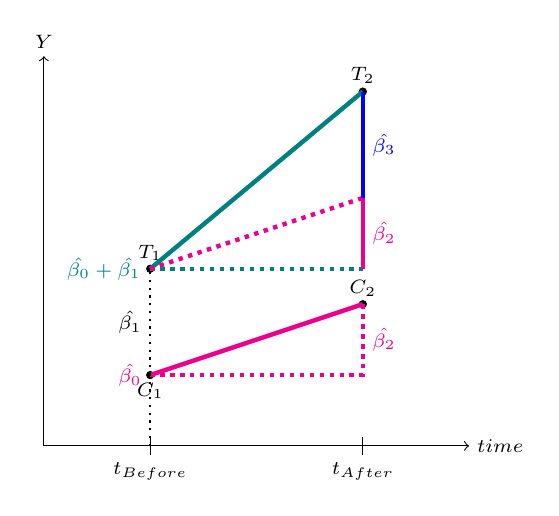
\begin{tikzpicture}[scale=.45]\scriptsize 
				\draw[->] (-1,0) -- (11,0) coordinate (x axis) node[right]{$time$};
 				\draw[->] (-1,0) -- (-1,11) coordinate (y axis) node[above]{$Y$};	
 				\draw[fill=black](2,2)circle(0.1cm)node[below]{$C_1$};
 				\draw[fill=black](8,4)circle(0.1cm)node[above]{$C_2$};
 				\draw[fill=black](2,5)circle(0.1cm)node[above]{$T_1$};
 				\draw[fill=black](8,10)circle(0.1cm)node[above]{$T_2$};
            	\draw[ultra thick, magenta] (2,2)--(8,4);
            	\draw[ultra thick, dotted, magenta] (2,2)--(8,2)--node[right]{$\hat{\beta_2}$}(8,4);
            	\draw[ultra thick, teal] (2,5)node[left]{$\hat{\beta_0}+\hat{\beta_1}$}--(8,10);
            	\draw[ultra thick, dotted, teal] (2,5)--(8,5);
            	\draw[ultra thick, magenta](8,5)--node[right]{$\hat{\beta_2}$}(8,7);
            	\draw[ultra thick, dotted, magenta](2,5)--(8,7);
            	\draw[ultra thick, blue](8,7)--node[right]{$\hat{\beta_3}$}(8,10);
            	\draw (2,0.25)--(2,-0.25)node[below]{$t_{Before}$};
            	\draw (8,0.25)--(8,-0.25) node[below]{$t_{After}$};
            	\draw[thick, dotted](2,2)--node[left]{$\hat{\beta_1}$}(2,5);
            	\draw[thick, dotted](2,0)--(2,2)node[left]{\textcolor{magenta}{$\hat{\beta_0}$}};
 			\end{tikzpicture}	
	\end{figure}
	\begin{equation*}
	\Delta \Delta Y= (Treated_{after}-Treated_{before})-(Control_{after}-Control_{before})
	\end{equation*}
	\item OLS Coefficients: 
		\begin{itemize}
			\item $\hat{\beta_0}$: value of $Y$ for control before treatment 
			\item $\hat{\beta_1}$: difference between treatment and control (before treatment)
			\item $\hat{\beta_2}$: time difference between before and after treatment
			\item $\hat{\beta_3}$: difference-in-difference: effect of treatment    
		\end{itemize}
	\item Values of $Y$ for different groups:
		\begin{itemize}
			\item $Y$ for Control Group Before: $\hat{\beta_0}$
			\item $Y$ for Control Group After: $\hat{\beta_0}+\hat{\beta_2}$
			\item $Y$ for Treatment Group Before: $\hat{\beta_0}+\hat{\beta_1}$
			\item $Y$ for Treatment Group After: $\hat{\beta_0}+\hat{\beta_1}+\hat{\beta_2}+\hat{\beta_3}$
			\item Treatment Effect: \textcolor{blue}{$\hat{\beta_3}$}
		\end{itemize}
	\item Key assumption about \emph{counterfactual}: if not for treatment, the treated group would change the same over time as the control group (parallel time trends, magenta dotted line)
	\item Can generalize the model with  two way fixed effects: 
	\begin{equation*}
\widehat{Y_{it}}=\alpha_i +\tau_t+\beta_3 (\text{Treated}_i \times \text{After}_{t})+ X_{it}+\epsilon_{it}	
\end{equation*}
	\begin{itemize}
		\item $\alpha_i$: group-fixed effects, where some groups receive treatment and others do not
		\item $\tau_t$: time-fixed effects, where some periods are before treatment and others are after
		\item $X_{it}$: other control variables 
		\item This allows for multiple treatments to happen at different times! 
	\end{itemize}
\end{itemize}
\end{itemize}
\clearpage 

\section*{Instrumental Variables}
\begin{itemize}
	\item A variable $IV$ can act as an instrumental variable if: 
	\begin{enumerate}
				\item Inclusion Condition: $IV$ statistically significantly explains $X$
				\begin{equation*}
				corr(X, IV) \neq 0	
				\end{equation*}
				\item Exclusion Condition: $IV$ doesn't directly affect $Y$ (not in $\epsilon$)
				\begin{equation*}
				corr(Y, IV) = 0	
				\end{equation*}
	\end{enumerate}
	\item $IV$ only affects $Y$ \emph{through} its relationship with $X$
	\item $IV$ removes endogenous variation of $X$ (correlated with $\epsilon$) and only uses \emph{exogenous} variation of $X$ (correlated with $IV$ but not with $\epsilon$) to estimate causal effect of $X \rightarrow Y$ 
	\item Implement in regression with Two Stage Least Squares (2SLS)
	\begin{enumerate}
		\item First Stage (Auxiliary Regression)
		\begin{equation*}
		\widehat{X_{1i}}=\widehat{\gamma_0}+\widehat{\gamma_1}IV_i+\widehat{\gamma_2}X_{2i}+ \widehat{\nu_i}	
		\end{equation*}
		\begin{itemize}
			\item Use instrument and other control variables (e.g. $X_2$) to predict value of $X_{1i}$
			\item Can test the inclusion restriction by testing significance of $\gamma_1$ ($|t$-statistic$|>3$)
		\end{itemize}
		\item Second Stage 
		\begin{equation*}
				\widehat{Y_i}=\hat{\beta_0}+\hat{\beta_1}\widehat{X_{1i}}+\hat{\beta_2}X_{2i}+ \widehat{\epsilon_i}		
		\end{equation*}
		\begin{itemize}
			\item Use the predicted value of $\widehat{X_{1i}}$ from First Stage 
			\item There is no statistical test for the exclusion restriction, must argue why $IV$ does not affect $Y$ (except through $X$)
		\end{itemize} 
	\end{enumerate}

\end{itemize}

\end{document}
